\chapter{Future Directions}
\label{ch:future}

This chapter identifies emerging technologies, research directions, and funding pathways that could extend and scale the approach developed in this pilot project. The landscape of 3D reconstruction and neural rendering is evolving rapidly; several developments anticipated in 2026--2027 have the potential to substantially advance the capabilities described in this report.

\section{CoMe: Confidence-Based Mesh Extraction}
\label{sec:fut-come}

CoMe (Confidence-based Mesh Extraction) \parencite{Radl2025CoMe} represents a significant methodological advance over existing mesh extraction approaches. By computing per-region confidence scores from the Gaussian representation and adapting mesh resolution accordingly, CoMe promises to address the uniform-quality-loss problem that characterises current methods: high-confidence regions (well-observed surfaces) receive fine tessellation, while low-confidence regions (poorly observed or geometrically complex areas) are represented more conservatively, reducing artefacts.

At the time of writing, the CoMe implementation has not been publicly released. The authors have indicated a release timeline coinciding with the CVPR 2025 conference proceedings. Upon release, CoMe should be integrated into the \texttt{gaussian-toolkit} pipeline and evaluated against the existing \acrshort{tsdf} and MILo extraction methods.

The confidence-based approach is particularly relevant to cultural heritage applications, where reconstruction quality varies significantly across the scene---well-covered gallery walls versus poorly observed ceiling regions, for example. A confidence-aware mesh could provide an honest representation of reconstruction certainty, which is valuable metadata for archival purposes.

\section{Multi-View Generation for Object-Level Reconstruction}
\label{sec:fut-hunyuan}

Tencent's Hunyuan3D-2.0 \parencite{Zhao2025Hunyuan} demonstrates the emerging capability of generating consistent multi-view images from a single input photograph or text description. While current-generation models do not achieve the geometric fidelity required for preservation applications, the trajectory of improvement suggests that within 1--2 generations, multi-view generation could serve as a powerful augmentation for under-observed regions of a scene.

The application scenario is as follows: given a cultural heritage scene where certain objects or regions were inadequately captured (insufficient viewpoints, occluded surfaces), a multi-view generation model could synthesise plausible additional views to improve reconstruction completeness. This would not replace direct capture but could provide a valuable fallback for historical recordings where re-capture is impossible.

\section{SAM3 for Automated Scene Decomposition}
\label{sec:fut-sam3}

The integration of third-generation Segment Anything models with 3D reconstruction pipelines is an active area of development. SAM3's ability to produce 3D-consistent segmentations from multi-view images---identifying the same object across all views without manual annotation---enables fully automated scene decomposition.

For cultural heritage, automated decomposition would allow a single walkthrough capture to be automatically parsed into individual objects, each of which could be:

\begin{itemize}
  \item Catalogued independently in a collection management system.
  \item Reconstructed at higher quality through targeted re-processing.
  \item Associated with existing catalogue records through visual similarity matching.
  \item Exported for individual study, 3D printing, or re-contextualisation.
\end{itemize}

The combination of automated segmentation with the splat-as-artefact approach (Section~\ref{sec:rec-primary}) would create a powerful workflow: capture a space once, automatically decompose it into objects, and deliver both the whole-scene experience and individual object access through a single browser-based interface.

\section{EU Horizon 2027 Alignment}
\label{sec:fut-horizon}

The European Commission's Horizon Europe programme has consistently prioritised cultural heritage digitisation, with Cluster 2 (Culture, Creativity and Inclusive Society) providing dedicated funding streams. The 2027--2028 work programme is expected to include calls related to:

\begin{itemize}
  \item AI-assisted digitisation of cultural heritage collections.
  \item Virtual access to cultural heritage for inclusion and education.
  \item Standards and interoperability for 3D cultural heritage data.
  \item Cross-border digital heritage infrastructure.
\end{itemize}

The \texttt{gaussian-toolkit} pipeline and the findings of this pilot project provide a strong foundation for a competitive Horizon Europe proposal, particularly if combined with:

\begin{enumerate}
  \item A consortium of European cultural institutions with complementary collections and preservation needs.
  \item Academic partners in computer vision, HCI, and digital humanities.
  \item Industry partners providing scalable cloud infrastructure and viewer technology.
\end{enumerate}

The University of Salford's existing international partnerships and the pilot project's demonstrated results position it well as a coordinator or key participant in such a consortium.

\begin{recommendation}
DreamLab AI and the University of Salford should begin consortium development for a Horizon Europe proposal in Q3 2026, targeting the anticipated Cluster 2 calls in the 2027--2028 work programme. The pilot project results provide essential preliminary data demonstrating feasibility and impact potential.
\end{recommendation}

\section{Scaling to Multiple Venues}
\label{sec:fut-scaling}

The current pilot has demonstrated the pipeline's viability for a single gallery space. Scaling to multiple venues---across the University of Salford's facilities, partner institutions, and external cultural heritage sites---requires addressing several practical considerations:

\begin{description}
  \item[Cloud processing infrastructure.] Local \acrshort{gpu} processing is sufficient for individual captures but does not scale to institutional-level throughput. A cloud-based processing backend---leveraging GPU instances from AWS, GCP, or Azure---would enable parallel processing of multiple captures and eliminate the dependency on local hardware.

  \item[Standardised capture training.] A training programme for cultural heritage practitioners, covering the capture methodology guidelines in Section~\ref{sec:rec-capture}, would ensure consistent input quality across diverse capture personnel and venues.

  \item[Collection management integration.] The splat viewer and associated metadata must integrate with existing collection management systems (e.g., Axiell Collections, TMS, ResourceSpace) to ensure that preserved 3D content is discoverable and manageable within established institutional workflows.

  \item[Long-term storage and format migration.] Gaussian splat representations must be incorporated into institutional digital preservation strategies, with consideration for format longevity, bit-level preservation, and future format migration pathways.

  \item[Access control and rights management.] Cultural heritage content frequently carries complex rights considerations---artist moral rights, institutional reproduction rights, and data protection implications for spaces containing identifiable individuals. The delivery infrastructure must support appropriate access controls.
\end{description}

\begin{figure}[htbp]
  \centering
  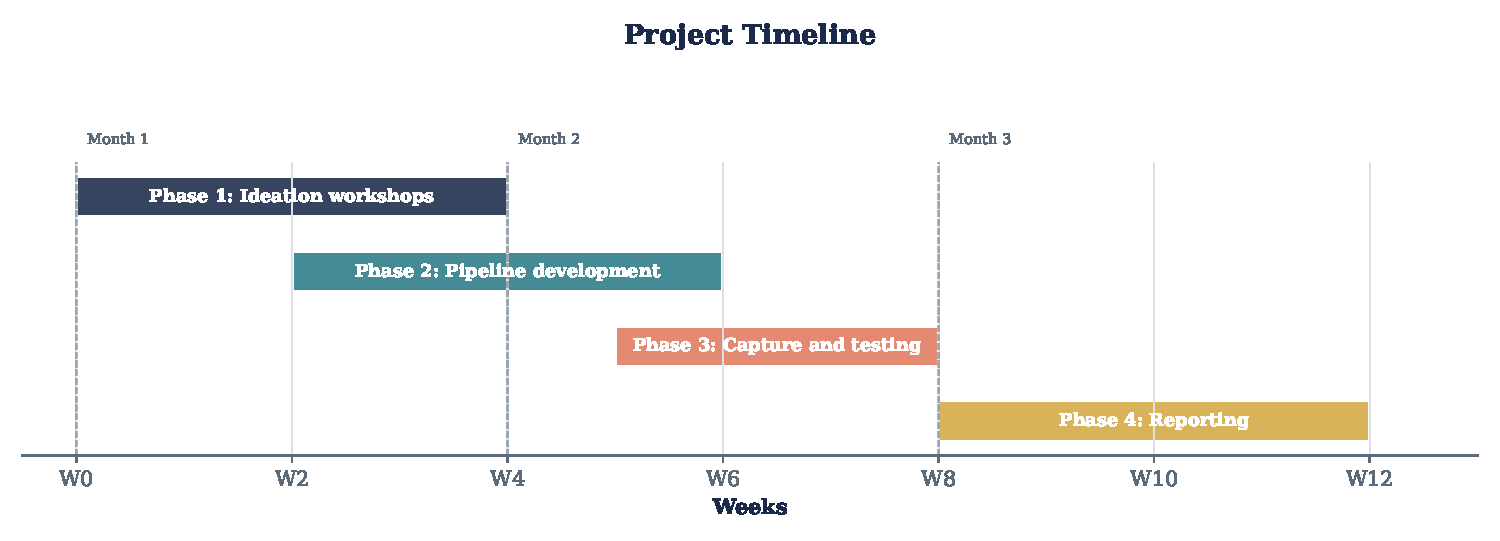
\includegraphics[width=0.85\textwidth]{figures/timeline.pdf}
  \caption{Proposed scaling roadmap from pilot to institutional deployment to consortium-level infrastructure.}
  \label{fig:scaling-roadmap}
\end{figure}
